\documentclass[a4paper,11pt,spanish,sans]{exam}
\usepackage[spanish]{babel}
%\usepackage[utf8]{inputenc}
\usepackage{multicol}
%\usepackage[latin1]{inputenc}
\usepackage{fontspec}%la posta para las tildes con lualatex
\usepackage[margin=0.5in]{geometry}
\usepackage{amsmath,amssymb}
\usepackage{multicol}
\usepackage{natbib}
\usepackage{graphicx}
\usepackage{hyperref}
\usepackage{epstopdf}
\usepackage{capt-of}
\usepackage[usenames]{color}


\newcommand{\class}{Matemática: Guía de  Funciones Irracional}
\newcommand{\term}{2° Trimestre 2015}
\newcommand{\examnum}{Tema 1}
\newcommand{\examprof}{Alexis Gomel}
\newcommand{\examdate}{15/7/2015}
\newcommand{\timelimit}{60 Minutes}%no lo uso

%el header de las hojas.
\pagestyle{head}
\firstpageheader{}{}{}
\runningheader{\class}{\examnum\ - Page \thepage\ of \numpages}{\examdate}
\runningheadrule


\begin{document}


\noindent
\begin{tabular*}{\textwidth}{l @{\extracolsep{\fill}} r @{\extracolsep{6pt}} l}
\textbf{\class} & \textbf{Profesor: \examprof}\\

%\textbf{Time Limit: \timelimit} & Teaching Assistant & \makebox[2in]{\hrulefill}
\end{tabular*}\\
\rule[2ex]{\textwidth}{2pt}

%%%%%%%%%%%%%%%%%%%%%%%%%%%%%%%%%%%%%%%%%%%
%Temas: Racional, Proporcionalidad inversa. Homografica, analisis y construccion. Ecuaciones e inecuaciones. Funcion Irracional. Ecs irracionales. (entran rufinni?, div de polinomios? etc...¿¿¿¿????, meto algo de limites?????; entra el modulo??)



\section*{Algunos ejemplos graficos de Logaritmos}

Definición de función irracional: Es cuando la función  presenta un radical . Es decir que tiene algun termino que se escribe como : 
\[ f(x)=\sqrt[n]{g(x)}\]
Donde g(x) es una función racional..

Ejemplo: $ f(x)= \sqrt(x)$; $g(x)=\sqrt[3]{x^2+x+5}$; $\sqrt[4]{log(x)}$

%    Si el índice n de la raíz es impar, es posible calcular la imagen de cualquier número real, siempre y cuando la expresión g(x) sea un número real, es decir, Dom(f)=Dom(g).
%    Si el índice n de la raíz es par, para poder calcular imágenes necesitamos que g(x) sea positiva o cero, ya que las raíces pares de un número negativo no son números reales. Por tanto el dominio de f son las soluciones de la inecuación g(x)≥0. En otras palabras, Dom(f)={x∈R∣g(x)≥0}.
%

%Estudiemos ahora el caso más simple de función irracional: la función raíz cuadrada f(x)=x√.
%
%Se trata de una función en que el índice de la raíz es 2. Por tanto, su dominio es el conjunto de soluciones de la inecuación x≥0. Así tenemos Dom(f)=[0,+∞) La imagen de la función raíz cuadrada es, como en el caso del dominio, el conjunto de los reales mayores o igual que cero, Im(f)=[0,+∞)
%

\begin{figure}[h!]
\centering
\includegraphics[width=0.7\textwidth]{raiz.jpg}
\caption{}
\label{fig:coplogs}
\end{figure}

\begin{figure}[h!]
\centering
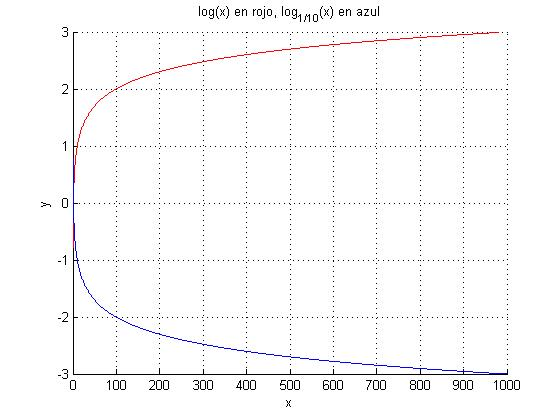
\includegraphics[width=0.7\textwidth]{amboslog10.jpg}
\caption{Graficos de $log(x)$ y $log_{\frac{1}{10}}(x)$.}
\label{fig:amboslogs}
\end{figure}

Si se traban con algún ejercicio, pasen al siguiente, y vuelvan al ejercicio difícil mas tarde.

\section{Graficos:}
Graficar las siguientes funciones , indicando raíces, dominio, imagen y si son biyectivas (en cuyo caso encontrar la inversa y su dominio).

\begin{enumerate}%cambiar funcion

\item $f(x)=-\sqrt{x}$
\item $f(x)=\sqrt{x-1}$
\item $f(x)=\sqrt{x+1}$
\item $f(x)=\sqrt{1-x^2}$
\item $f(x)=\sqrt[3]{x-1}$


\section{Resolver las siguientes ecuaciones, especificando que restricciones son necesarias :}

\begin{enumerate}
\begin{multicols}{2}

\item $\sqrt{1-x}=\sqrt{x^2-5}$
\item $x+2=13-\sqrt{x-5}$
\item $\sqrt{x^2-5 +7 = x^2}$%ojo con este a ver si sale o no.
\item $x^2+\sqrt{x^2+9}=21$
\item $\sqrt{x+1}+\sqrt{2x+3}-\sqrt{8x+1}=0$

\end{multicols}
\end{enumerate}


\section*{Extra}

%El numero $e\simeq$ ..  breve bio de euler-
\begin{itemize}
\item 

\item 

\item 

\begin{figure}[h!]
\centering
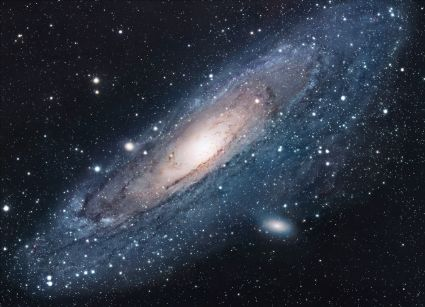
\includegraphics[scale=1.7]{universe.jpg}
\caption{The Universe}
\label{fig:univerise}
\end{figure}

\end{itemize}

%\bibliographystyle{plain}
%\bibliography{references}
\end{document}
%%%%%%%%%%%%%%%%%%%%%%%%%%%%%%%%%%%%%%%%%%%
%Temas: Racional, Proporcionalidad inversa. Homografica, analisis y construccion. Ecuaciones e inecuaciones. Funcion Irracional. Ecs irracionales. (entran rufinni?, div de polinomios? etc...¿¿¿¿????, meto algo de limites?????; entra el modulo??)
